\documentclass[onecolumn, draftclsnofoot, 10pt, compsoc]{IEEEtran}
\usepackage{graphicx}
\usepackage{url}
\usepackage{setspace}
\usepackage{geometry}

\geometry{textheight=9.5in, textwidth=7in}

% @here - we should consider modifying this, it looks kind of weird and lacks some of the info I'd like to have + this year's logo
% 1. Fill in these details
\def \CapstoneTeamName{			Team 12}
\def \CapstoneTeamNumber{		12}
\def \GroupName{				CS Capstone Team }
\def \GroupMemberOne{			Trey Elkins}
\def \GroupMemberTwo{			Leif Tsang}
\def \GroupMemberThree{			Ryan Wallerius}
\def \CapstoneProjectName{		NASA USLI Rocket Team}
\def \CapstoneSponsorCompany{	Oregon State University}
\def \CapstoneSponsorPerson{	Dr. Nancy Squires}

% 2. Uncomment the appropriate line below so that the document type works
\def \DocType{		%Problem Statement
					Requirements Document
					%Technology Review
					%Design Document
					%Progress Report
				}
			
\newcommand{\NameSigPair}[1]{
	\par
	\makebox[2.75in][r]{#1} \hfill
	\makebox[3.25in]{\makebox[2.25in]{\hrulefill} \hfill \makebox[.75in]{\hrulefill}}
	\par\vspace{-12pt}
	\textit{
		\tiny\noindent \makebox[2.75in]{} \hfill
		\makebox[3.25in]{\makebox[2.25in][r]{Signature} \hfill \makebox[.75in][r]{Date}}
	}
}
% 3. If the document is not to be signed, uncomment the RENEWcommand below
\renewcommand{\NameSigPair}[1]{#1}
\renewcommand{\thesubsubsection}{\thesection.\alph{subsubsection}}

%%%%%%%%%%%%%%%%%%%%%%%%%%%%%%%%%%%%%%%
\begin{document}
\begin{titlepage}
    \pagenumbering{gobble}
    \begin{singlespace}
    	%\includegraphics[height=4cm]{coe_v_spot1}
        \hfill 
        % 4. If you have a logo, use this includegraphics command to put it on the coversheet.
        %\includegraphics[height=4cm]{CompanyLogo}
        \begin{center}
           
\includegraphics[scale = 0.4]{osu_usli_logo.png}\\[1.0 cm]

        \par\vspace{.2in}
        \scshape{
            \huge CS Capstone \DocType \par
            {\large\today}\par
            \vspace{.5in}
            \textbf{\Huge\CapstoneProjectName}\par
            \vfill
            {\large Prepared for}\par
            %\Huge \CapstoneSponsorCompany\par
            \vspace{5pt}
            {\Large\NameSigPair{\CapstoneSponsorPerson}\par}
            {\large Prepared by }\par
           	\GroupName\par
            % 5. comment out the line below this one if you do not wish to name your team
            %\CapstoneTeamName\par
            \vspace{5pt}
            {\Large
                \NameSigPair{\GroupMemberOne}\par
                \NameSigPair{\GroupMemberTwo}\par
                \NameSigPair{\GroupMemberThree}\par
            }
            \vspace{20pt}
        }
        \end{center}
    \end{singlespace}
    
    \begin{abstract}
    	% 6. Fill in your abstract
        This document outlines the client requirements for the computer science portion of the Oregon State University's entry into the NASA University Student Launch Initiative. The systems outlined in this requirements document entail rocket tracking and avionics, rover payload operations, and management of the team website.
	\end{abstract}
\end{titlepage}
\newpage

\pagenumbering{arabic}
\tableofcontents
% 7. uncomment this (if applicable). Consider adding a page break.
%\listoffigures
%\listoftables
\clearpage


%\section*{Revision History}
%\begin{center}
	%\begin{tabular*}{1\linewidth}{@{\extracolsep{\fill}}|c|c|c|c|}
        %\hline
	    %Name & Date & Reason For Changes & Version\\
        %\hline
        %J.Novak, A.Sladek, L.Willmeth & 10/26/17 & Initial document draft & 0.1 \\
        %\hline
	    %J.Novak, A.Sladek, L.Willmeth & 4/29/18 & Updates to reflect hardware changes & 0.2 \\
        %\hline
    %\end{tabular*}
%\end{center} 

\section{Project Overview}
\subsection{Introduction}
The NASA Student Launch is a research-based, competitive, experiential exploration and learning activity. It strives to provide relevant, cost-effective research and development in the field of rocket propulsion and launch systems. This project offers multiple challenges reaching a broad audience of middle and high schools, colleges, and universities across the United States.

\subsection{Purpose}
This document outlines the customer and competition requirements for the Computer Science team participating in Oregon State University's entry into the NASA Student Launch Initiative.

\subsection{Scope}
The software described in this document will support the Oregon State University (OSU) American Institute of Aeronautics and Astronautics (AIAA) team's entry for the NASA Student Launch Initiative competition taking place in April 2019. 

% @here - this sucks, let's fix it?
\subsection{Definitions, acronyms, and abbreviations}
\begin{center}
  \begin{tabular}{|l|l|}
      \hline
      AIAA	&American Institute of Aeronautics and Astronautics\\
      CS		&Computer Science\\
      \hline
      ECE		&Electrical and Computer Engineering\\
      ME		&Mechanical Engineering\\
      \hline
      OSU		&Oregon State University\\
      \hline
  \end{tabular}
\end{center}

% @here - this also sucks
\subsection{References}
\subsection*{Initial Project Description}
https://www.nasa.gov/audience/forstudents/studentlaunch/home/index.html\\
NASA Student Launch\\
https://oregonstate.instructure.com/courses/1692930/assignments/7282754\\
CS capstone Requirments Document\\
https://github.com/OSU-USLI-19/CS-Capstone-2018-2019-Team-Documents

\subsection{Overview}
This document contains the complete software requirements and specifications for the computer science portion of the NASA University Student Launch Initiative.  The software can be organized into three parts:

\begin{enumerate}
\item \textbf{Launch Vehicle Avionics and Telemetry}, a system that actively tracks, logs, and forwards coordinate (GPS) flight data. 
\item \textbf{Payload Software}, must maneuver 10 feet away from the landed rocket with object avoidance and collect a soil sample specified by the competition requirements.
\item \textbf{Website}, the location where NASA will receive design and technical documents required for the competition as well as a place to display other information and facts about the team.
\end{enumerate}

This document has been updated to reflect changes in customer requirements specified by NASA personnel and the team administration over the course of the competition.

% @here - we need to make sure formatting is consistent with IEEE standard and/or what we've been doing for our other assignments, ex. add \noindent if necessary

% @here - wow this section is absolutely boned, we need to figure out how we want to split it out
\section{Overall description}
\subsection{Product perspective}
The launch vehicle avionics system will collect and log coordinate data from on-board GPS sensors. Data will be used for analysis of launch vehicle flight profile and drift radius for reporting in NASA documentation, as well as for recovery of the launch vehicle after flight.

The rover payload will use sensors to implement object avoidance. The program will be written and managed by the CS team. The CS team will be in contact with the ECE team on decisions made for payload management and operations. 

The Website will not be graded in the competition itself but is crucial for storage and retrieval of key technical documentation required by NASA for competition purposes. The Website will be managed and created by the CS team and will be published on a domain purchased by the OSU USLI Team. 

\subsubsection{System interfaces}
The launch vehicle avionics software will interact with the GPS sensors and data logging via a Teensy 3.6 microcontroller running Arduino code. 

% @here - Leif do you want to strip the BeagleBone stuff out or keep it in and we can discuss in the final report why we aren't using it?
\noindent The payload software will control the rover through both a Teensy 3.6 and BeagleBone Black microcontroller.

\noindent The Website will be hosted on a domain purchased by the OSU USLI team via the Github.io web service.

% @here we're missing rover interfaces
\subsubsection{Hardware interfaces}
The rocket avionics will interact with GPS sensors on-board the rocket to collect coordinate data during the flight. The Teensy will manage an XBee Pro S3 900 MHz transceiver that packs filtered data and sends it to a ground station utilizing similar hardware for data output and recovery purposes. The flight units are equipped with SD cards that log the data to text files for later recovery and analysis. 

% @here - ?????
\subsubsection{Software interfaces}
External libraries or software may be used to create graphs from information in the database.

The rocket avionics program will read and write to a local database.

\subsubsection{Memory constraints}
Avionics software must comply with memory constraints of the Teensy 3.6 as well as buffer and serial constraints of the XBee Pro S3 transceiver. Serial monitors and scripts can be run on Windows machines or any other computer that has support for standard programming languages.

% @here - rover??

% @here - website??

\subsection{Product functions}
\subsubsection{Rocket Avionics functions}
Read coordinate data from GPS sensors.\\
Log and filter GPS data.\\
During flight, rocket avionics units will transmit data to ground station. \\
After flight, ground station transmits trigger signal to payload ejection controller. \\

% @here - consistent formatting, also lets update this
\subsubsection{Payload functions}
Read data from individual sensors.

Be able to properly use object avoidance. 

Drive at least ten feet away from the landed rocket and collect a soil sample. 

\subsection{User characteristics}
The intended users of these systems will be primarily ECE and CS team members - typically college-aged students familiar with software and high level electronics. The primary exception to this is the website, which will need to be navigable and easily usable by any adult, though the real target users will be NASA engineers, members of other teams, and potential sponsors who are curious about our team and documentations.

\subsection{Constraints}
\subsubsection{Regulatory policies}
Competition restrictions dictate that our approach to various problems must be different in order to accommodate competition requirements. Everything must comply with federal law and with the requirements enumerated in the Student Launch Initiative handbook.

\subsubsection{Interfaces to other applications}
Outside of situations such as radio-frequency interference, our systems must not interrupt or compromise the operation of any other team's systems at competition. In cases where all interaction cannot be eliminated - such as in use of commonplace radio-frequency bands - measures must be taken to minimize impact on the systems of other teams.

\subsubsection{Control functions}
Control functions are limited by hardware limitations due to airframe dimensions or ejection requirements, as well as by hardware chosen to perform said control operations.

\subsubsection{Higher-order language requirements}
Both the rocket avionics and rover payload software must be written in a high level programming language such as the Arduino programming language. The website must also be implemented using tools or libraries other than just basic HTML, CSS, and JavaScript.

% @here - this is BS
\subsubsection{Safety and security considerations}
The rocket will launch far enough away from spectators not to pose a safety threat.

% @here - lol nah
\subsection{Assumptions and dependencies}
The ECE/ME team will provide the computer hardware necessary to run the Rocket and Payload Programs. 

The ECE team will provide the CS team with sufficient time and information to test and debug our software using their final version of the flight hardware.

% @here - this needs heavy revisiting
\section{Specific requirements}
\subsection{System features}
\subsubsection{Avionics features}
The Avionics code needs to be cleaned up and have efficiency improved. 

They will likely be written in C or a higher level language

The Avionics programs will be thoroughly tested. This program must store critical flight data and be retrievable. 

\subsubsection{Payload Software}
The rover must move at least ten feet away from the landed rocket

The rover must avoid any objects in its path

The rover must collect a soil sample it see's acceptable 

\subsubsection{Website}
The website must store critical documents for NASA's retreival. 

\subsection{Development Chart Timeline}
\begin{center}
  \makebox[\textwidth]{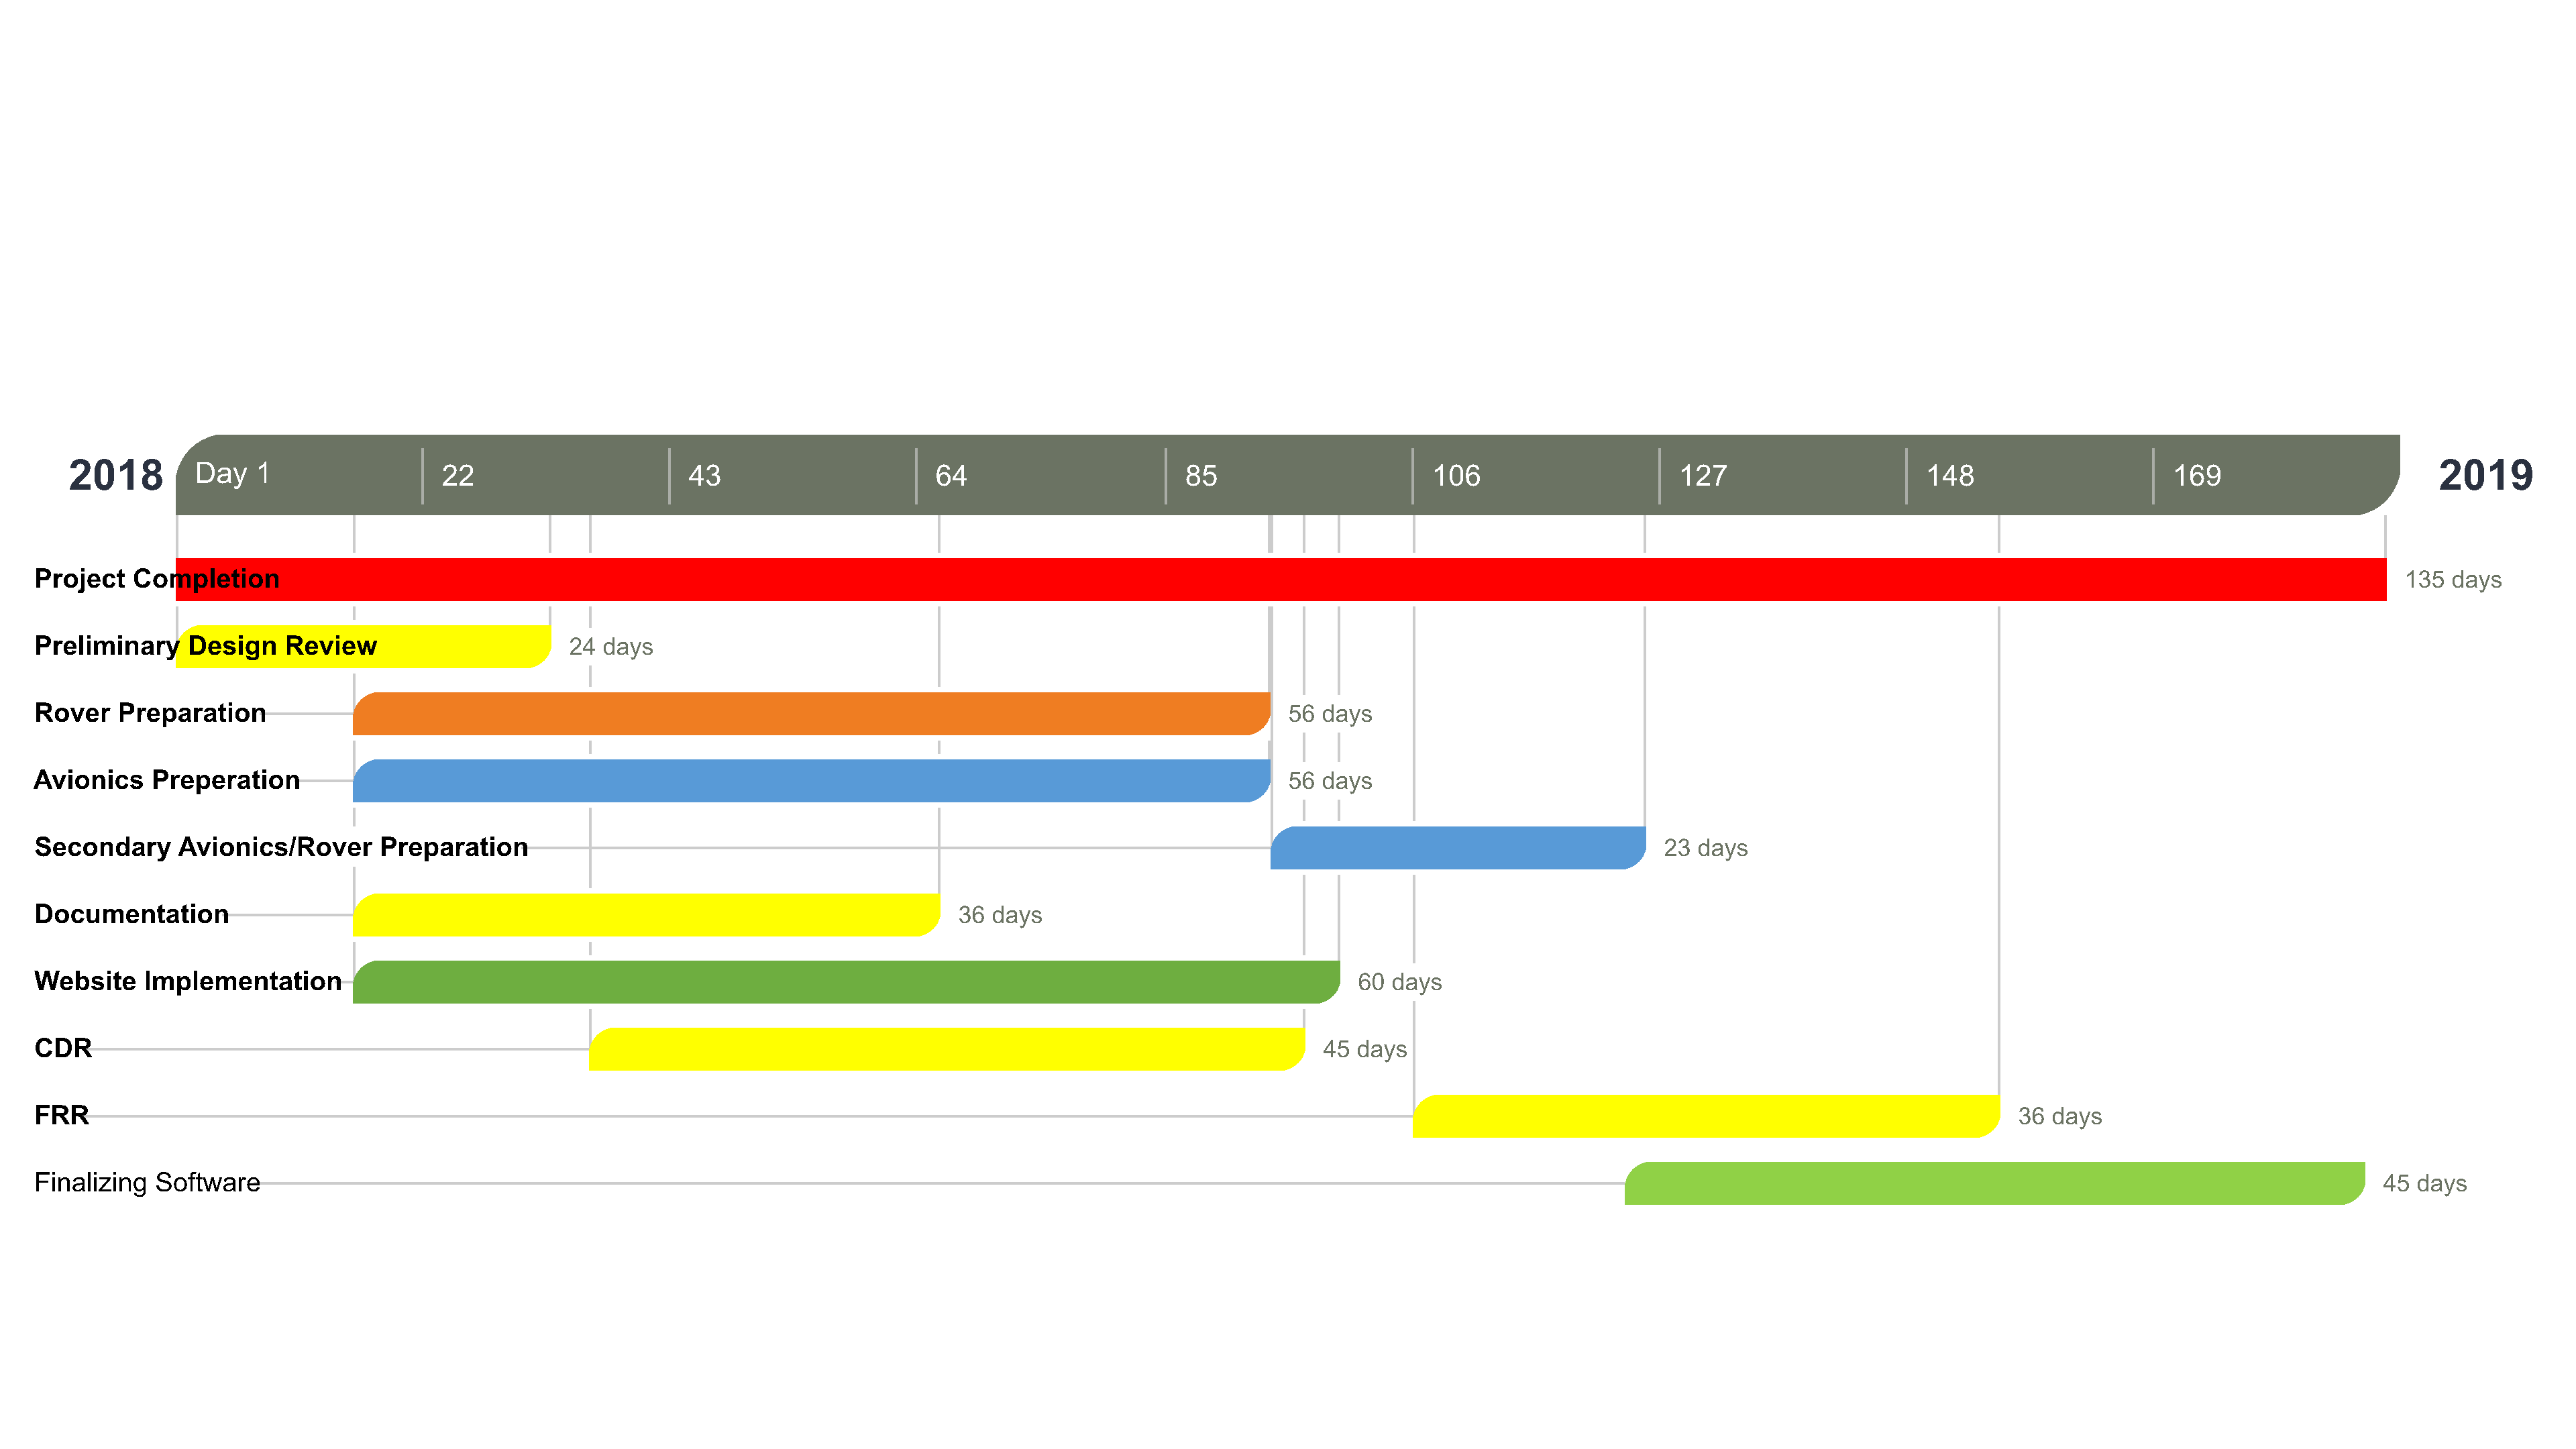
\includegraphics[width=\paperwidth]{PlanningRoadmap.png}} 
\end{center}


\end{document}